% This code uses the tikz package
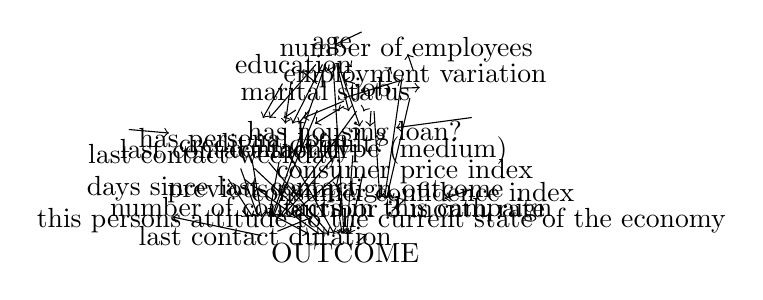
\begin{tikzpicture}
\node (v0) at (0.829,-0.313) {consumer confidence index};
\node (v1) at (0.722,-0.0510) {consumer price index};
\node (v2) at (0.258,0.218) {contact type (medium)};
\node (v3) at (-0.829,0.309) {credit in default?};
\node (v4) at (-1.59,-0.270) {days since last contact};
\node (v5) at (0.853,1.16) {employment variation};
\node (v6) at (0.889,-0.517) {euribor 3 month rate};
\node (v7) at (0.0850,0.432) {has housing loan?};
\node (v8) at (-1.24,0.345) {has personal loan?};
\node (v9) at (-1.05,-0.877) {last contact duration};
\node (v10) at (-1.45,0.231) {last contact month};
\node (v11) at (-1.70,0.131) {last contact weekday};
\node (v12) at (-0.287,0.973) {marital status};
\node (v13) at (-0.210,-0.533) {number of contacts in this campaign};
\node (v14) at (0.740,1.50) {number of employees};
\node (v15) at (-0.159,-0.300) {previous campaign outcome};
\node (v16) at (0.425,-0.679) {this persons attitude to the current state of the economy};
\node (v17) at (-0.0340,-1.09) {OUTCOME};
\node (v18) at (-0.203,1.54) {age};
\node (v19) at (-0.689,1.31) {education};
\node (v20) at (0.314,0.993) {job};
\draw [->] (v0) edge (v16);
\draw [->] (v1) edge (v16);
\draw [->] (v2) edge (v9);
\draw [->] (v2) edge (v17);
\draw [->] (v3) edge (v9);
\draw [->] (v3) edge (v17);
\draw [->] (v4) edge (v9);
\draw [->] (v4) edge (v17);
\draw [->] (v5) edge (v16);
\draw [->] (v5) edge (v20);
\draw [->,<-] (v5) edge (v14);
\draw [->] (v6) edge (v16);
\draw [->] (v7) edge (v3);
\draw [->] (v7) edge (v9);
\draw [->] (v7) edge (v17);
\draw [->] (v8) edge (v3);
\draw [->] (v8) .. controls (-1.23,0.209) and (-1.17,-0.198) .. (v9);
\draw [->] (v8) edge (v17);
\draw [->,<-] (v9) edge (v17);
\draw [->] (v10) edge (v9);
\draw [->] (v10) edge (v17);
\draw [->] (v11) edge (v9);
\draw [->] (v11) edge (v17);
\draw [->] (v12) edge (v3);
\draw [->] (v12) edge (v7);
\draw [->] (v12) edge (v8);
\draw [->] (v12) edge (v9);
\draw [->] (v13) edge (v9);
\draw [->] (v13) edge (v17);
\draw [->] (v14) edge (v16);
\draw [->] (v14) edge (v20);
\draw [->] (v15) edge (v9);
\draw [->] (v15) edge (v13);
\draw [->] (v15) edge (v17);
\draw [->] (v16) edge (v17);
\draw [->] (v18) edge (v2);
\draw [->] (v18) edge (v3);
\draw [->] (v18) edge (v7);
\draw [->] (v18) edge (v8);
\draw [->] (v18) edge (v9);
\draw [->] (v18) edge (v12);
\draw [->] (v18) edge (v17);
\draw [->] (v18) edge (v19);
\draw [->] (v18) edge (v20);
\draw [->] (v19) edge (v3);
\draw [->] (v19) edge (v8);
\draw [->] (v19) edge (v12);
\draw [->] (v19) edge (v20);
\draw [->] (v20) edge (v2);
\draw [->] (v20) edge (v3);
\draw [->] (v20) edge (v7);
\draw [->] (v20) edge (v8);
\draw [->] (v20) edge (v9);
\draw [->] (v20) edge (v12);
\draw [->] (v20) edge (v16);
\end{tikzpicture}